%%%%%%%%%%%%%%%%%%%%%%%%%%%%%%%%%%%%%%%%%%%%%%%%%%%%%%%%%%%%%%%%%%%%
\section{Data Acquisition System (DAQ) Overview (Georgia Karagiorgi and Dave Newbold)}
\label{sec:fdsp-daq-ov}

%\metainfo{2 Pages - largely generic but some highlighting of SP-specifics.}

%%%%%%%%%%%%%%%%%%%%%%%%%%%%%%%%%
\subsection{Introduction}
\label{sec:fdsp-daq-intro}

The DUNE Far Detector (FD) Single-Phase Data Acquisition (DAQ) System
design must enable the readout, processing and distribution to
permanent storage of physics and calibration data from each 10~kton SP
module, including data from the PD, TPC, accelerator and timing,
calibration, and other auxiliary systems.
An overview of the overall DUNE FD DAQ System is illustrated in
Fig.~\ref{fig:daq-overview}. 
Figure~\ref{fig:daq-overview} illustrates the main DAQ subsystem
components as well as the data flow and the exchange of trigger and
monitoring messages between them.
As shown, it is applicable to both TPC and PD system readout, except
that in the case of the PD system the DAQ scope begins to the right of
the Front-End Readout. 
%\fixme{Describe figure here.}

\begin{dunefigure}[DAQ Overview]{fig:daq-overview}
  {A generalized overview of high-level far detector \dword{daq}
    components showcasing the \dword{sp} \dword{detmodule}. 
    The electronics digitizes the detector signals and sends the data
    to the DAQ \dword{fe} readout hardware which sends the data to the
    \dword{fe} computing data receiver.
    The \dword{fe} readout hardware also processes the data stream to
    produce \dwords{trigprimitive} which are sent along with the data
    itself.
    The receiver sends the data to the \dword{ringbuffer} which is of
    sufficient size to retain the data long enough for a
    \dword{trigcommand} formed from the data itself to return.
    The receiver is also responsible to send out
    \dwords{trigcandidate}, formed from the \dwords{trigprimitive}, to
    the \dword{mtl} as input to forming a \dword{trigcommand}. 
    The \dword{mtl} forwards notification of this trigger process and
    accepts external \dwords{trigcandidate} from the \dword{gtl}.
    \Dwords{trigcommand} are then sent to the \dlong{eb} which queries
    the appropriate \dword{fe} computing units, aggregates the
    returned data and writes it to the \dword{diskbuffer} which is the
    interface to the Offline.}
% This PDF is made from the .dot of the same name.
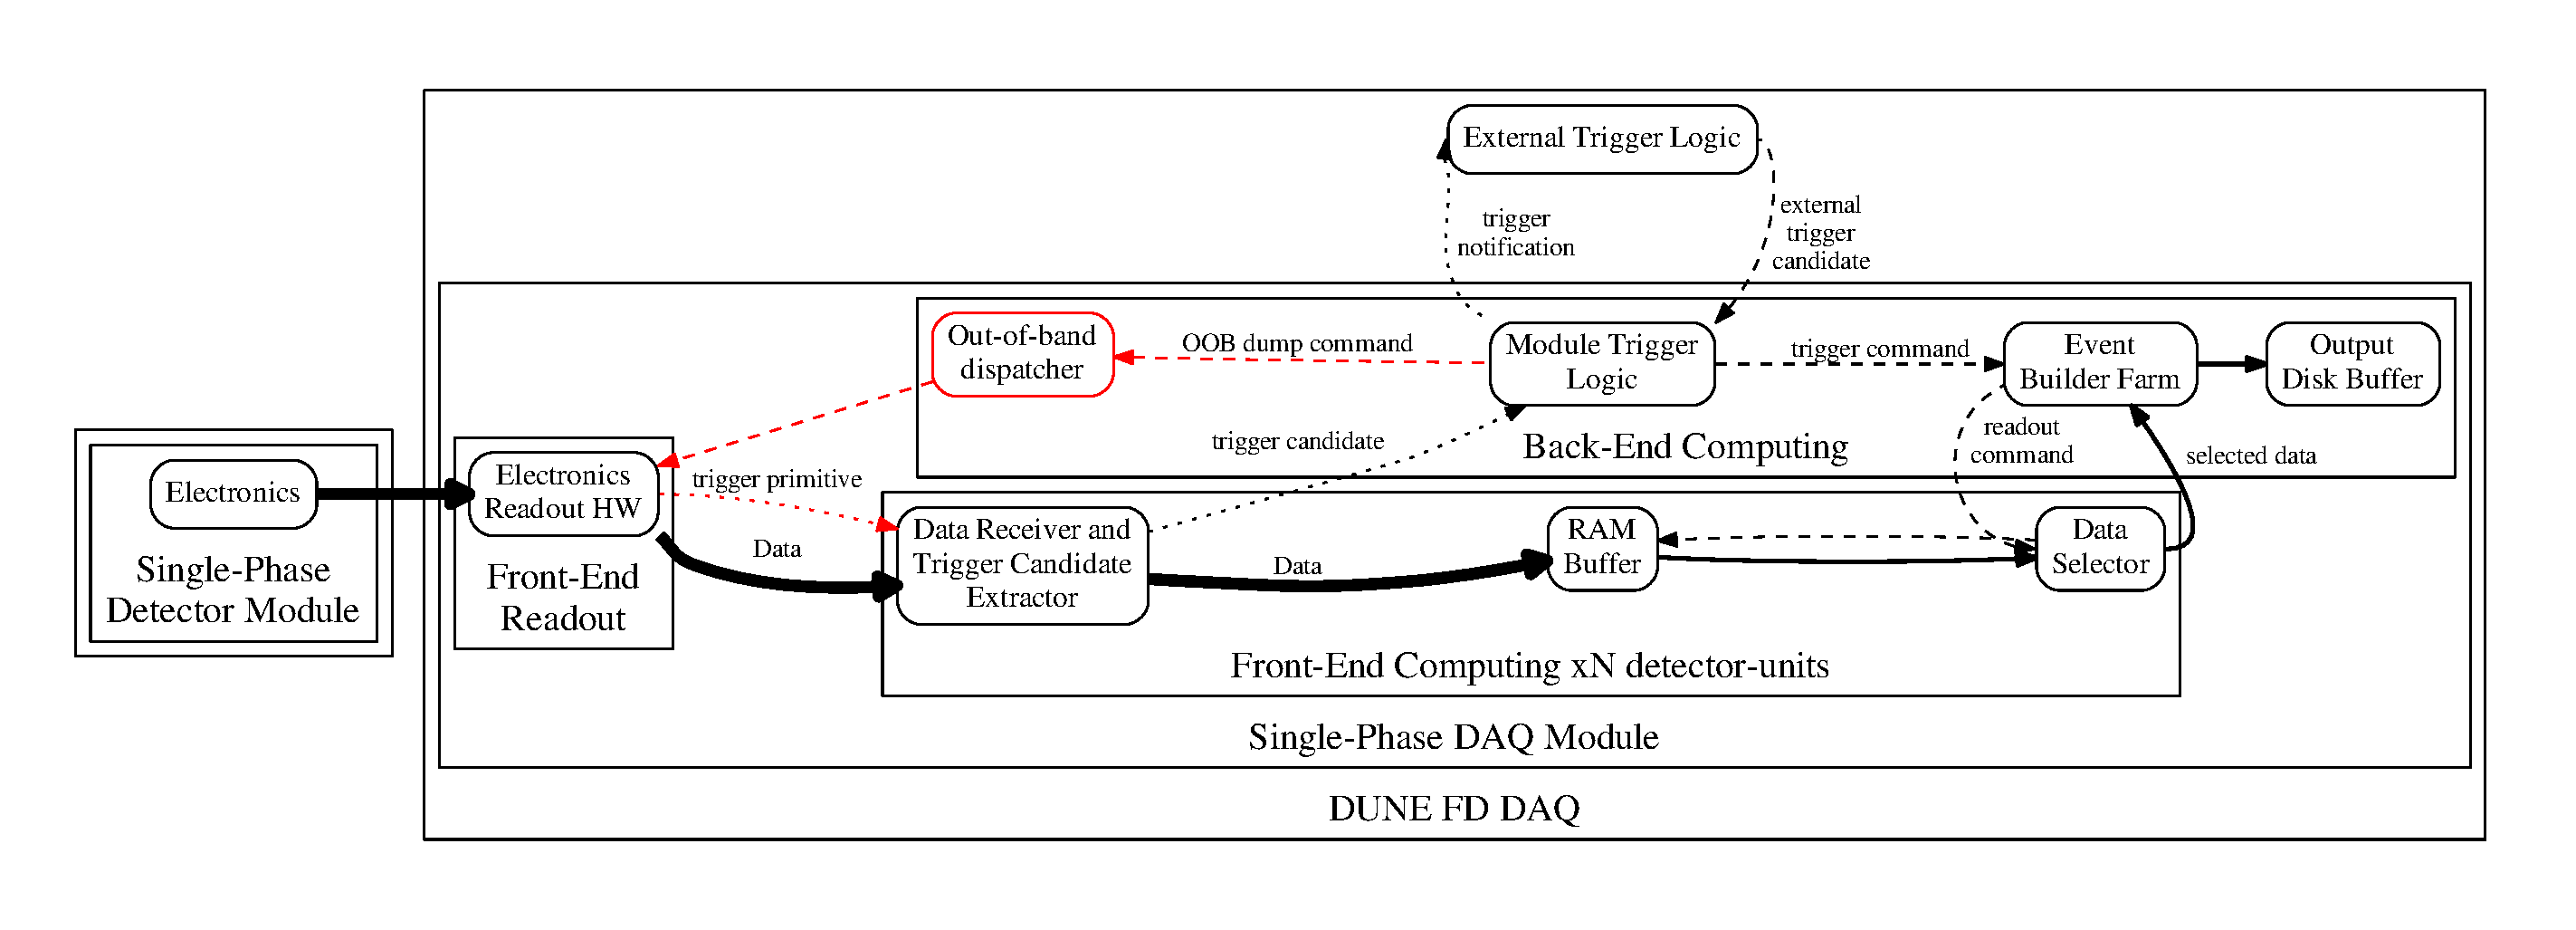
\includegraphics[width=0.8\textwidth]{daq-overview-sp.pdf}%
\end{dunefigure}


%%%%%%%%%%%%%%%%%%%%%%%%%%%%%%%%%%%%%

\subsection{Design Considerations}
\label{sec:fdsp-daq-des-consid}


%\metainfo{Include: Raw data rate from WIBs, Josh's table of data volumes for each event type and the 30 PB/year offline limit. Space and thermal power limits.  Note, this table may be better put into Section~\ref{sec:fdsp-daq-design} to make this section more generic.}

%\fixme{Anne suggests: Within this section add ref to requirements document when it's ready, and maybe list the most important half dozen in a table here). E.g.,}  
The high level requirements for the DUNE FD DAQ are provided in
\cite{daq:reqs}.
The most critical requirements in consideration for the overall design
are summarized in Tab.~\ref{tab:daqrequirements}.

The data rates and thus the processing needs of the DAQ are expected
to be dominated by the TPC system.
In particular, the DAQ must be designed to handle (receive, process,
compress, select, and hand off to back-end computing) raw TPC data
rates of up to \SI{6.14}{\TB/\s}. 
This rate assumes:
\begin{itemize}
\item Four (4) \SI{10}{\kton} Single Phase (SP) TPC detector modules
\item 150 Anode Plane Assemblies (APAs) per module
\item 2560 wire channels per APA 
\item 2 MHz digitization rate
\item 2 Bytes per sample (note that this is an overestimate, as data will be digitized with a 12-bit ADC)
\end{itemize}
\fixme{We need to standardize plane labeling throughout, there are three standards (also u/v/w, u/v/x and u/v/y).}

A back-end requirement is that the total volume of physics data that
can be shipped to off-site data centers for offline analysis is
limited to \SI{100}{\Gbps}.
An additional requirement is that a year’s worth of data amounts to no
more than \SI{30}{\PB} of data to permanent disk per year for the
entire DUNE FD, including all four (4) \SI{10}{\kton}
\dwords{detmodule} (each including TPC, PD system, calibration
systems, etc.).

The anticipated interaction rates due to the anticipated source for
the full FD are summarized in Tab.~\ref{tab:daqdatarates}. 
These rates assume noise levels are as expected from intrinsic
electronics noise.
Excess noise such as due to \dword{rf} emission inside the cryostat
would lead to an overwhelming trigger rate if left unmitigated.
An \dword{trigdecision} in the DUNE FD concerns:
\begin{enumerate}
\item \Dwords{trigcandidate} derived from the data from the \dword{detmodule} itself.
\item \Dwords{externtrigger} injected from trigger sources outside the \dword{detmodule} context.
\item \dword{snb} \dword{trigcommand} derived from \dword{detmodule} \dwords{trigcandidate} or from cross-module or SNEWS \dwords{externtrigger}
\end{enumerate}
When executing a \dword{trigcommand} data blocks continguous in time
and channel over a \dword{detmodule} will be saved. 
For the \dword{sb} \dword{detmodule} the nominal block is \readout in
time and covers all TPC channels and associated \dword{pds}. 
This is chosen to encompass two drift times with a modest additional
padding.
The nominal \dword{snb} readout window is \snbtime and its ``dump''
includes all channels.  
Acquiring and \dword{snb} dump inflicts no subsequent dead time for
nominal data taking.
This is an overly conservative approach, and it is expected that with
better understanding of detector performance after commissioning and
initial operations this readout scheme will be improved to reduce data
volume further.

\begin{dunetable}
[Important requirements on the DAQ system design]
{ccc}
{tab:daqrequirements}
{Important requirements on the DAQ system design}   
Requirement  & Description \\ \toprowrule
Scalability & The DUNE FD DAQ shall be capable of receiving and
buffering the full raw data from all four FD modules \\ \colhline 
Zero deadtime & The DUNE FD DAQ shall operate without deadtime under
"normal" operating conditions \\ \colhline
Triggering & The DUNE FD DAQ shall provide full-detector triggering
functionality as well as self-triggering
functionality; the data selection shall maintain high efficiency to
physics events while operating within a total bandwidth of 30 PB/year
for all operating FD modules \\ \colhline
Synchronization & The DUNE FD DAQ will provide synchronization of
different FD modules to within 1~$\mu$s, and of different subsystems
within a module to within 10~ns\\ \colhline
\end{dunetable}

\begin{dunetable}
[Anticipated event and data rates in the DUNE FD]
{llp{0.8\textwidth}}
{daq:datarates}
{Anticipated event and data rates in the DUNE FD assuming all four
  modules are SP. The
  rates assume continuous readout (without any data reduction) for
  5.4~ms for non-extended events, and for 10 seconds for extended events.}   
Event Type  & Annual Data Volume & Assumptions \\ \toprowrule
 Beam interactions & 27 TB & 800 beam and 800 dirt muons; 10~MeV
 threshold in coincidence with beam time; include cosmics\\ \colhline
 Cosmics and atmospherics & 10 PB &  \\ \colhline
 Radiologicals & $\le$1~PB & fake rate of $\le$100 per year \cite{daq:simreport}\\ \colhline
 Front-end calibration & 200~TB & Four calibration runs per year, 100
 measurements per point \\ \colhline
 Radioactive source calibration & 100~TB & source rate $\le$10~Hz;
 single APA readout; lossless readout \\ \colhline
 Laser calibration & 200~TB & 1$\times$10$^6$ total laser
 pulses, lossy readout \\ \colhline
 Random triggers & 60 TB & 45 per day\\ \colhline
 Trigger primitives & $\le$6~PB &  all three wire planes; 12 bits per
 primitive word; 4 primitive quantities; $^{39}$Ar-dominated\\ \colhline




%\fixme{By the end of the volume, for every requirement listed in this section, there should exist an explanation of how it will be satisfied.}


%%%%%%%%%%%%%%%%%%%%%%%%%%%%%%%%
\subsection{Scope}
\label{sec:fdsp-daq-scope}

%\metainfo{This section may also wish to refer to Fig.~\ref{fig:daq-overview}.}

The scope of the \dword{daq} system includes the continued procurement
of materials for, and the fabrication, testing, delivery and
installation of the following systems:

\begin{itemize}
\item Readout electronics (only for TPC)
\item Front-end computing servers, including disk 
\item Back-end computing servers, including disk
\item External trigger hardware 
\item Data selection algorithms
\item Timing distribution system
\item DAQ firmware for readout electronics
\item DAQ data handling software including receiving and building of
  events
\item Run control software, configuration database, and user interface
\item Rack infrastructure in the central utility cavern for readout
  electronics, front-end computing, timing distribution, and data
  selection
\item Rack infrastructure on surface at SURF for back-end computing
\end{itemize}


